\chapter{Theoretische Grundlagen}
\label{background}

%- Allgemeine Wissensgrundlagen des Fachgebiets
%- Spezielle Grundlagen, die für das Verständnis erforderlich sind
%- Rahmenbedingungen für die Arbeit
%- Ausführungen zum Stand des Wissens / der Technik
%Als Leitprinzip gilt: Nur Informationen erwähnen, die
%- später benötigt werden,
%- notwendig sind, um die Arbeit oder ihre Motivation zu verstehen
%Das heißt insbesondere,
%- keine Inhalte aus Lehrbüchern, außer
%- diese werden benötigt, um Problemstellung oder Lösungsweg zu definieren.

Ziel des nachfolgenden Kapitels soll es sein, eine allgemeine Wissensgrundlage über wesentliche Begrifflichkeiten im Thema zu schaffen. Um die nachfolgenden Ausführungen im Hauptteil (vgl. \ref{problemfields} und \ref{agilepractices}) besser nachvollziehen zu können, sollen wichtige Definitionen und Begriffsabgrenzungen vorgenommen werden.

\section{Digitale Transformation}

Der wesentliche Schwerpunkt der vorliegenden Arbeit dreht sich um die sogenannte Digitale Transformation. Eine allgemeine Definition für diese Begrifflichkeit ist momentan schwer zu finden \cite<vgl.>[S. 3]{schallmo_digitale_2017}. Grundsätzlich versteht man unter der Digitalen Transformation von Unternehmen den Einfluss neuer Technologien und Innovationen auf gesamtunternehmerische Strukturen, Geschäftsmodelle und Wertschöpfungsketten \cite<vgl.>{oswald_digitale_2018}. Nach \citeA{kofler_digitale_2018} sei es das Ziel der digitalen Transformation, Unternehmen fortlaufend und ohne vorhersehbares Ende so umzubauen, dass sie sich den kontinuierlichen Marktveränderungen durch Digitalisierung stellen können (S. 1). Man erkennt hierbei das Muster, dass die Begrifflichkeit der \textit{Digitalisierung} ein wichtiger Faktor für den strategischen Aufbau von Unternehmen geworden ist. Neue Innovationen im digitalen Bereich machen es vor allem kleineren Firmen einfacher in bestehende Märkte einzutreten und sogenannte \textit{Disruptionen} \todo{Erklärung als Fußnote} zu erschaffen. 
 
 
 Viele Versuche einer Definition betreffen immer den Bezug auf aufkommende digitale Technologien. Diese können als sogenannte \textit{Treiber} der Digitalen Transformation bezeichnet werden \cite<vgl.>[S.20]{bloching_digitale_2015}. \ref{fig:bigpicture} skizziert eine Übersicht dieser verschiedenen Treiber. Man erkennt hierbei schon wichtige Handlungsfelder des Transformationsprozess, wie beispielsweise die Automatisierung von Geschäftsprozessen oder die Nutzung von generierten Digitalen Daten. Solche Handlungsfelder werden in der vorliegenden Arbeit in \ref{problemfields:changepatterns} genauer erläutert.
 
\ref{fig:bigpicture} kennzeichnet außerdem, dass eine große Reihe von neuen Technologien die Digitale Transformation antreiben. Beispielsweise bilden Technologien wie \textit{Cloud Computing} oder \textit{Big Data} neue Möglichkeiten für digitalisierte Geschäftsmodelle. 
 
\begin{figure}[H]
	\centering
	\fbox{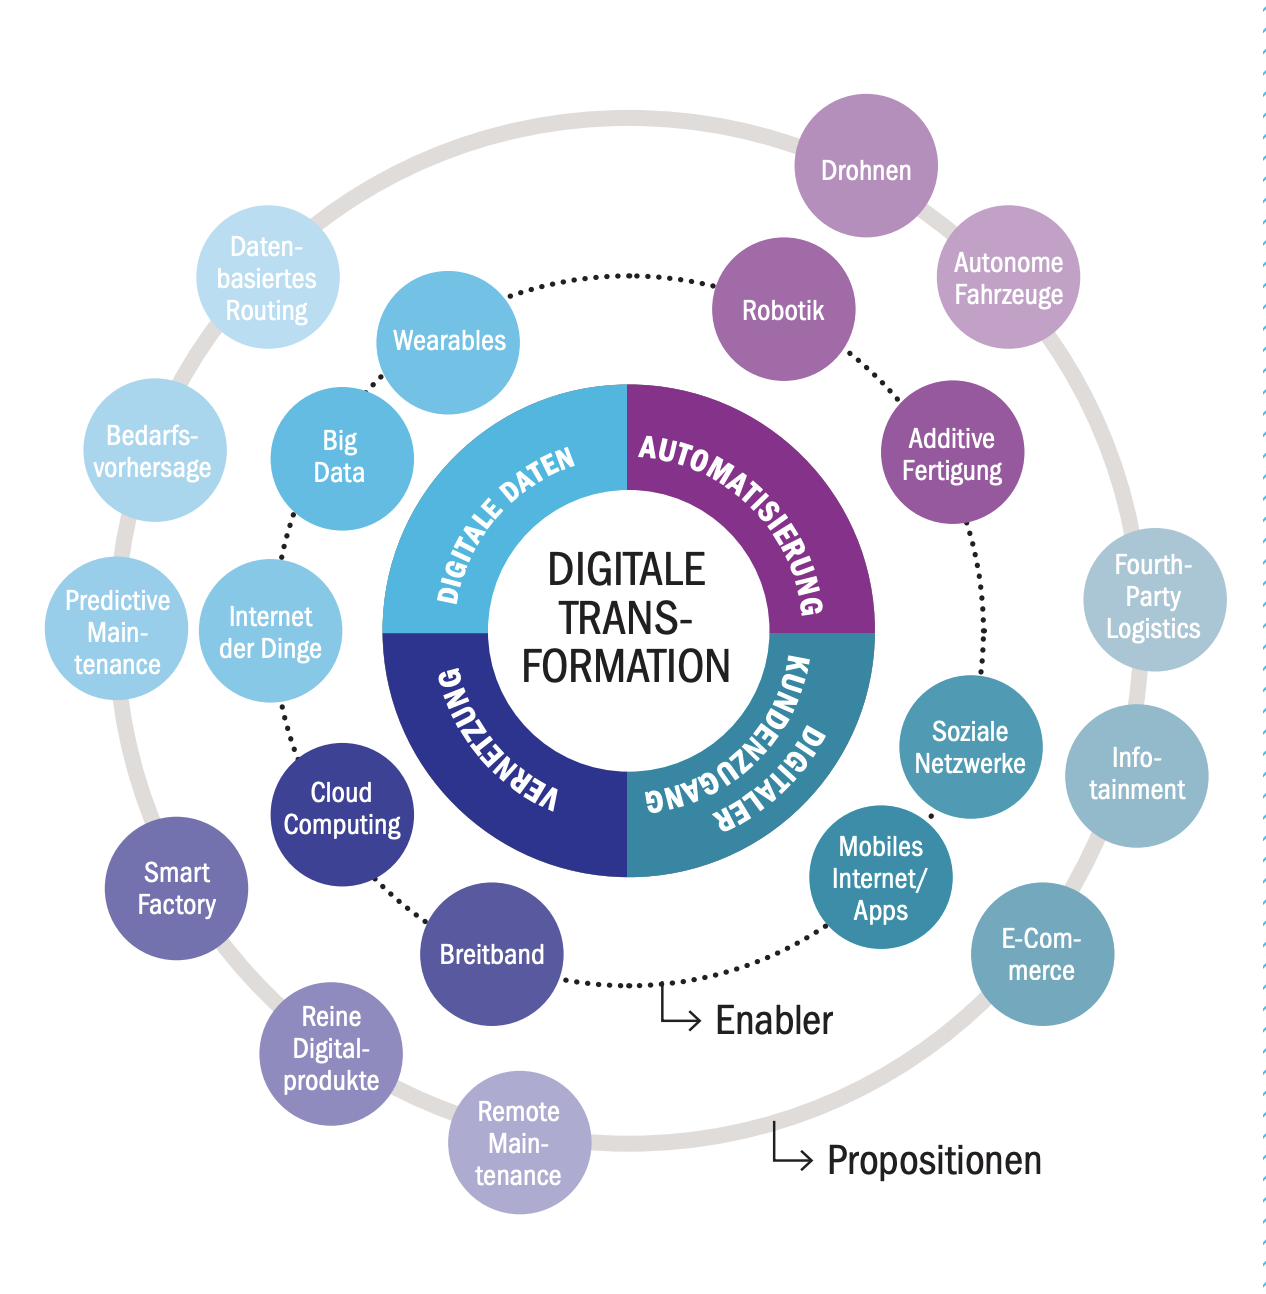
\includegraphics[width=0.7\linewidth]{pics/dtbigpicture}}
	\caption[Big-Picture der Digitalen Transformation]{Treiber der Digitalen Transformation \protect \cite[S. 20]{bloching_digitale_2015}}
	\label{fig:bigpicture}
\end{figure}

Die Digitale Transformation kann somit als weitreichender Veränderungsprozess von Unternehmen angesehen werden. \citeA{oswald_digitale_2018} beschreiben innerhalb dieses Prozesses vier bestimmende Charakteristika. Demnach sei die Digitale Transformation ''unausweislich, unumkehrbar, ungeheuer schnell und mit Unsicherheit behaftet`` (S. 10). Man erkennt hierbei also ein gewisses Risiko bei der Bearbeitung einer solchen Transformation. Es ginge für das Unternehmen vor allem darum, ''die Chancen neuer, digitaler Technologien kontinuierlich hinsichtlich ihres Potentials zur Weiterentwicklung bestehender Geschäftsmodelle zu evaluieren`` (S. 10).

Es kristallisiert sich ganz klar heraus, dass der Veränderungsprozess einer Digitalen Transformation zwar unausweichlich ist, um die eigene Marktposition zu verteidigen. Trotzdem zeigen sich zunehmende Risiken und Probleme bei der Implementierung solcher Veränderungen. Demnach liegt es nahe, sich in der vorliegenden Arbeit mit den Problemfeldern der Digitalen Transformation zu beschäftigen (vgl. \ref{problemfields}).

\section{Change Management}

Wie im vorhergehenden Abschnitt bereits angeklungen ist, handelt es sich bei der Digitalen Transformation um einen großangelegten Veränderungsprozess eines Unternehmens. Vordergründig kann definiert werden, dass es sich beim Veränderungsmanagement bzw. \textit{Change Management} um das ''$\lbrack$m$\rbrack$anagen von Veränderungen in Unternehmen und Organisationen`` \cite[S. 10]{kaune_change_2016} handelt. Durch die gravierenden Änderungen des Unternehmens und die Notwendigkeit, einen geordneten Veränderungsprozess anzustoßen, kann das Steuern der Digitale Transformation grundsätzlich als Change Management bezeichnet werden.

\todo{Kaune Kommunikation}
\todo{Agile Change Canvas}
\todots

\section{Agilität}

\todots

\section{Agile Organisation}

\todots

\section{Agile Transformation}

\todots

\section{Abgrenzung Großunternehmen}